\begin{answer}
\begin{figure}[H]
  \centering
  \vspace{2mm}
  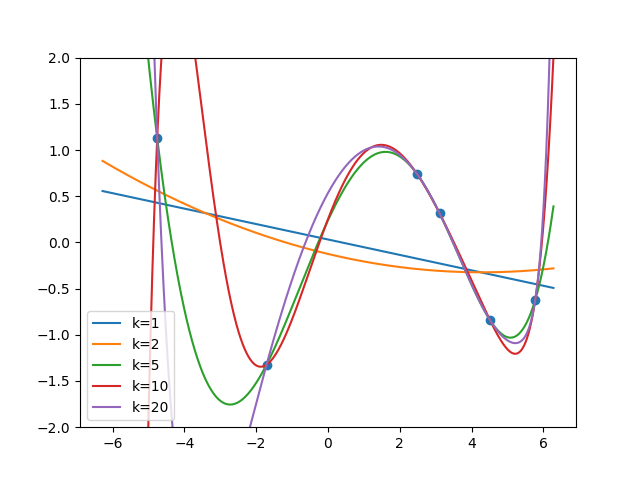
\includegraphics[width=0.65\linewidth]{../src/featuremaps/small-poly.png}
  \caption{Polynomial regression with kernel sizes 1,2,5,10 and 20
  on small dataset}
  \centering
  \vspace{2mm}
  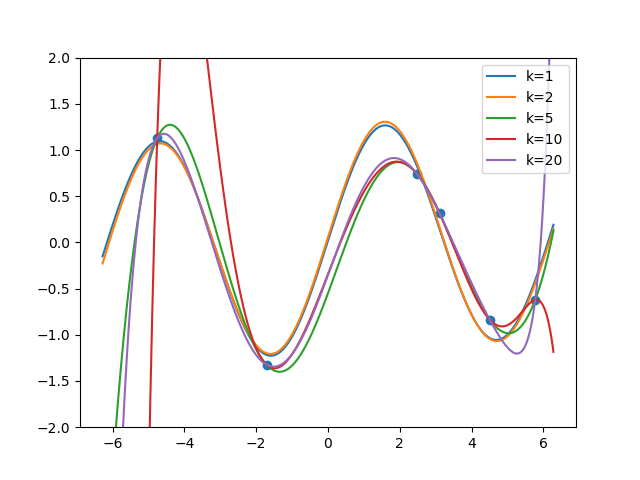
\includegraphics[width=0.65\linewidth]{../src/featuremaps/small-sine.png}
  \centering
\caption{Regression with other features with kernel sizes 1,2,5,10 and 20
on small dataset}

\end{figure}

We see that when the dataset is small, higher degree polynomials tend to pass through all the points, but qualitatively seem like a poor fit. Numerical instability with high degree polynomials remain a problem even with small data, with or without sin($x$).
\end{answer}
